% Sample University of Calgary Thesis
% This file contains the APPENDIX

% If there is just one appendix, it must be called ``Appendix.'' For
% multiple appendices, use \chapter and a descriptive title,
% e.g., \chapter{Questionnaires}

\chapter{Appendix~A: PprzTester documentations}\label{appendixa}

UML Diagrams and tables for the developed tools: flight data recorder, automated test generator, and automated test executor.
\begin{table}
    \centering
\begin{longtable}{llp{.50\columnwidth}}
\toprule
\textbf{Message Name }   & \textbf{Sent By }    & \textbf{Use}                                                                     \\ \hline
\endhead
%
\hline
\endfoot
%
\endlastfoot
%
PPRZ\_MODE &
  Aircraft &
  PprzTester listens to this message to find out when the auto-pilot software is booted up and is ready for flight. It also contains the state of active PID loops that is used to determine the internal state of the auto-pilot. \\
NAVIGATION &
  Aircraft &
  Contains the current active flight plan block as well as number of full circles the aircraft has completed among other data \\
COMMANDS        & Aircraft    & Contains commands from the auto-pilot to the servos (the outputs)       \\
FLIGHT\_PARAMS  & Aircraft    & Contains most of the sensor readings and required aircraft parameters   \\
ENGINE\_STATUS  & Aircraft    & Contains engine RPM and throttle among other parameters                 \\
CIRCLE\_STATUS &
  Aircraft &
  Contains detailed information about aircraft status while it is in circling mode. Overlaps with NAVIGATION to some extent \\
WAYPOINT\_MOVED & Server      & Sent in case any waypoints are relocated                                \\
MOVE\_WAYPOINT  & PprzTester & To update waypoint locations                                            \\
NEW\_AIRCRAFT &
  Server &
  Event of a new aircraft coming online in the network. It does not necessarily mean that it is ready for flight, should listen for PPRZ\_MODE as well \\
AIRCRAFTS\_REQ  & PprzTester & Request to get the list of active aircraft                              \\
AIRCRAFTS       & Server      & Response to the above request                                           \\
CONFIG\_REQ     & PprzTester & Request for an aircraft's configs                                       \\
CONFIG &
  Server &
  Response to the above request containing  its name, flight plan, DL settings, air frame parameters, etc. \\
DL\_SETTING     & PprzTester & Update a DL setting value. It is used to launch the aircraft in the air \\
JUMP\_TO\_BLOCK & PprzTester & Commands the aircraft to change active block to another block defined in the flight plan  \\ \bottomrule
\end{longtable}
\caption{Subset of all available messages in Paparazzi that are used in PprzTester tool}
\label{tab:pprz_messages}
\end{table}

\begin{table}
    \centering
\begin{longtable}{lp{.63\columnwidth}}
\toprule
\textbf{Argument}   & \textbf{Description}\\ \hline
\endhead
%
\hline
\endfoot
%
\endlastfoot
airframe              &  The aircraft to simulate \\
plan                  &  Plan name to run as a python module in \verb|pprz_tester.generated_plans| \\
--agent-name          &  Specify unique agent name on ivy bus \\
-l, --log             &  Log file directory \\
--log-format          &  The format to store and compress logs in, can be hd5 or csv \\ \hline
-p, --paparazzi-home  &  Directory in which Paparazzi source code is cloned in \\
-b,--build            &  Build the aircraft before launching the simulation \\
--gcs                 &  Open GCS window \\
--no-sim              &  Does not launch the simulator \\
--prep-mode           &  The required conditions before starting the flight scenario. It can be waiting for altitude to stabilize (climb) or waiting for a complete circle around stand by waypoint (circle) or both. \\ \hline
--fuzz-wps            &  Waypoints to fuzz locations of. Use * to fuzz all \\
--wp-fuzz-bounds-lat  &  Minimum and maximum latitude (south-north) to fuzz waypoint locations in \\
--wp-fuzz-bounds-lon  &  Minimum and maximum longitude (east-west) to fuzz waypoint locations in \\
--wp-fuzz-bounds-alt  &  The boundaries inside which waypoint altitudes are fuzzed \\
-w,--wp-location      &  Fix one or more waypoints' locations (overrides fuzzing) \\ \hline
-Dname=value          &  Optional plan arguments. They will be passed to \verb|get_items| as keyword arguments. \\ \bottomrule
\end{longtable}
\caption{Test runner command line arguments}
\label{tab:test_runner_commandline_args}
\end{table}


\begin{table}
    \centering
\begin{longtable}{lp{.63\columnwidth}}
\toprule
\textbf{Argument}   & \textbf{Description}\\ \hline
\endhead
%
\hline
\endfoot
%
\endlastfoot
airframe              &  The aircraft to generate tests for \\
output                &  Output file name or the directory to output the generated plans \\
-i, --include         &  Flight plan blocks to include in the generated plans \\
-x, --exclude         &  Flight plan blocks to exclude from the generated plans \\ 
-l, --length          &  Number of flight plan blocks to include. \\ \hline
-p, --paparazzi-home  &  \multirow{6}{*}{Shared with test runner in Table~\ref{tab:test_runner_commandline_args}}\\
--fuzz-wps            &   \\
--wp-fuzz-bounds-lat  &   \\
--wp-fuzz-bounds-lon  &   \\
--wp-fuzz-bounds-alt  &   \\
-w,--wp-location      &   \\ \bottomrule
\end{longtable}
\caption{Test runner command line arguments}
\label{tab:test_generator_commandline_args}
\end{table}


\begin{landscape}
\begin{figure}
    \centering
    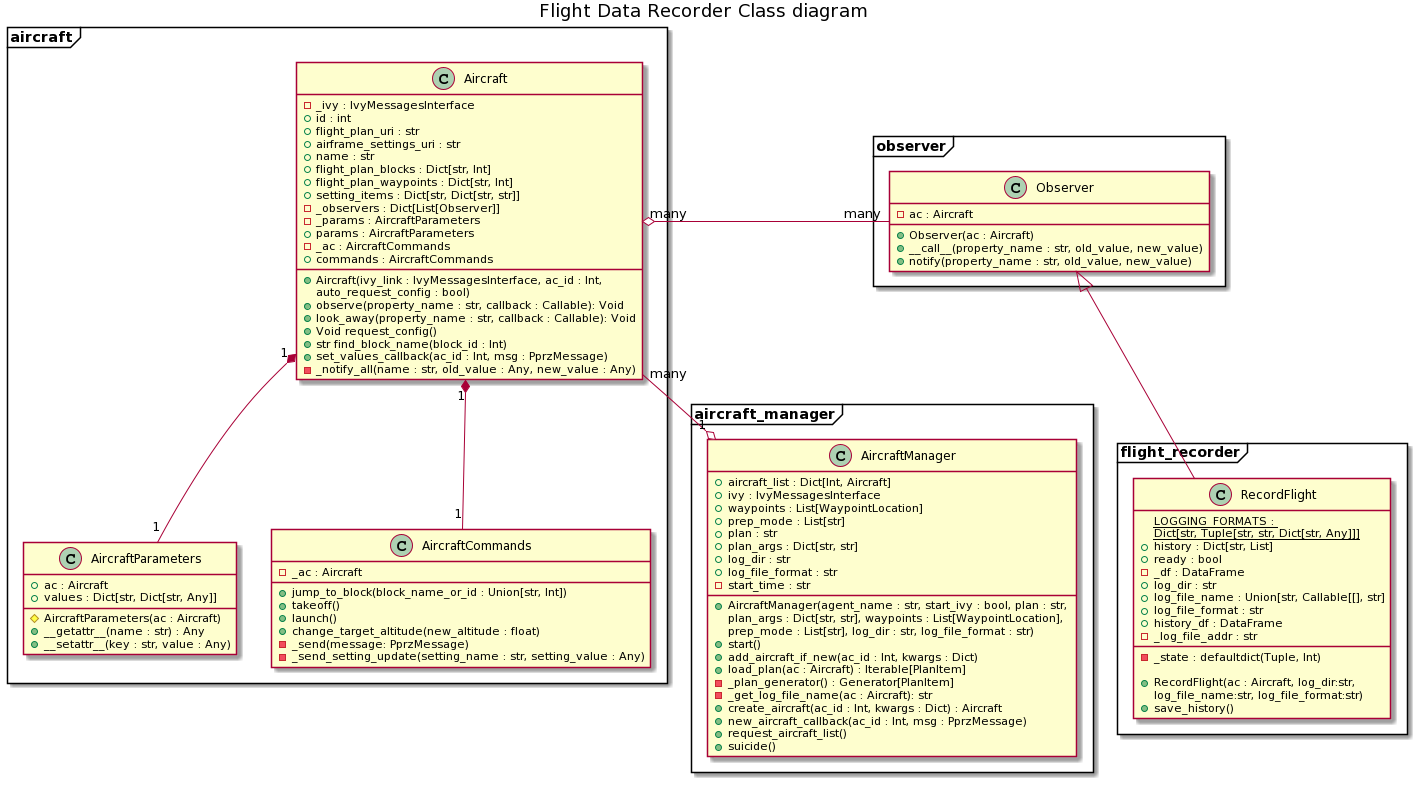
\includegraphics[width=\columnwidth]{pprz_tester_files/UML/fdr_class_diagram.png}
    \caption{Class diagram for flight data recorder}
    \label{fig:fdr_class_diagram}
\end{figure}
\end{landscape}

\begin{figure}
    \centering
    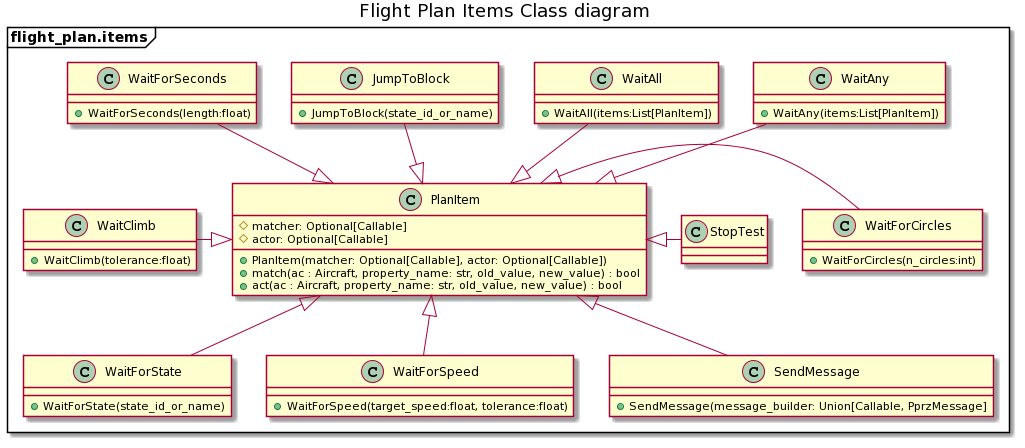
\includegraphics[width=\columnwidth]{pprz_tester_files/UML/flight_plan_items_class_diagram.png}
    \caption{Flight plan items}
    \label{fig:flight_plan_items_class_diagram}
\end{figure}

\begin{figure}
    \centering
    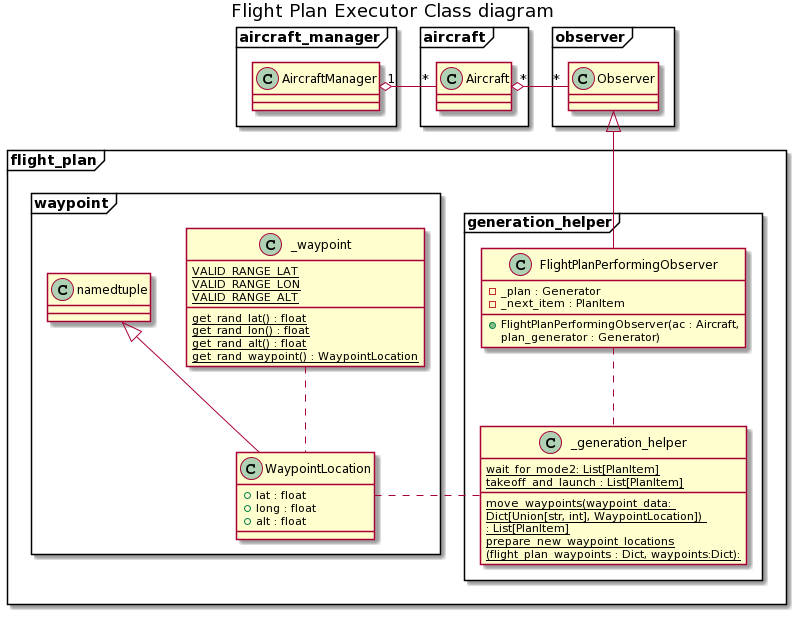
\includegraphics[width=\columnwidth]{pprz_tester_files/UML/flight_plan_executor_class_diagram.png}
    \caption{Flight executor classes}
    \label{fig:flight_plan_executor_class_diagram}
\end{figure}

\begin{landscape}
\begin{figure}
    \centering
    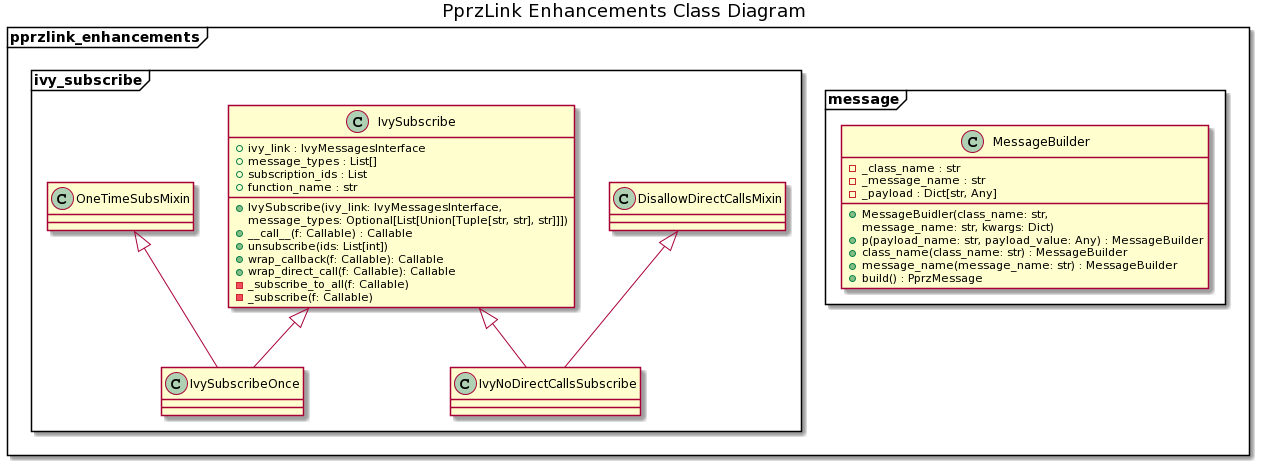
\includegraphics[width=\columnwidth]{pprz_tester_files/UML/pprzlink_enhancements_class_diagram.png}
    \caption{Class diagram for helpers and wrappers for PprzLink library}
    \label{fig:pprzlink_enhancements_class_diagram}
\end{figure}
\end{landscape}

\chapter{Appendix~B: Copyright}\label{appendixb}

\includegraphics[width=\textwidth]{Copyright.png}
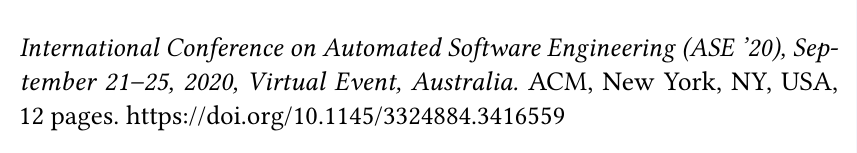
\includegraphics[width=\textwidth]{Copyright2.png}
I, as the author, retained the copyright to the above manuscript while licensing ACM for publication.
